\section{Experimental Results}
%
We have implemented ACDLP for bounded safety verification of C programs.  
ACDLP is implemented in C++ on top of the
\textsc{CPROVER}~\cite{cprover} framework and consists of around 9~KLOC. 
The template polyhedra domain is implemented in C++ in 10~KLOC.  Templates
can be intervals, octagons, zones, equalities, or restricted polyhedra.  Our
domain handles all C operators, including bit-wise ones, and supports
precise complementation of meet irreducibles, which is necessary for
conflict-driven learning.  Our tool and benchmarks are available 
at~\url{http://www.cprover.org/acdcl/}.
%


We verified a total of~85 ANSI-C benchmarks.  These are are derived from:
(1)~the bit-vector regression category in SV-COMP'16; (2)~ANSI-C models of
hardware circuits auto-generated by v2c~\cite{mtk2016} from VIS Verilog
models and opencores.org; (3)~controller code with varying loop bounds 
auto-generated from Simulink model and control 
intensive programs with nested loops containing relational properties. 
%The software models drawn from hardware benchmarks contains complex bit-wise
%operations, which are handled out-of-the-box by our domain implementation. 
All the programs with bounded loops are completely unrolled before
analysis.

We compare ACDLP with the state-of-the-art SAT-based bounded model checker
CBMC (\cite{cbmc}, version 5.5) and a commercial static analysis tool,
Astr{\'e}e (\cite{astree}, version 14.10).  CBMC uses MiniSAT~2.2.1 in the
backend.  Astr{\'e}e uses a range of abstract domains, which includes
interval, bit-field, congruence, trace partitioning, and relational domains
(octagons, polyhedra, zones, equalities, filter).  To enable fair comparison
using Astr{\'e}e, all bounded loops in the program are completely unwound up
to a given bound before passing to Astr{\'e}e.  This prevents Astr{\'e}e
from widening loops.
%
ACDLP is instantiated to a product of the Booleans
and the interval or octagon domain instance of template polyhedra.  ACDLP is
also configured with a decision heuristic (ordered, random, activity
based), propagation (forward, backward and multi-way), and conflict-analysis (learning UIP, DPLL-style).  The timeout for our experiments is set to one hour.  
%
\Omit {
To enable precise analysis using Astr{\'e}e, all our benchmarks are 
manually instrumented with partition directives which provides external 
hint to the tool to guide the trace partitioning heuristics.  Usually, 
such high-precision is not needed for static analysis, since it makes 
the analysis very expensive.  Without trace partitioning, the 
analysis using Astr{\'e}e shows high degree of imprecision. 
}

%%%%%%%%%%%%%%%%%%%%%%%%%% scatter plots %%%%%%%%%%%%%%%%%%%%%%%%%%%
\begin{figure}[t]
  \centering
\begin{tabular}{@{\hspace{-0.5em}}c@{\hspace{1.5em}}c}
\begin{tikzpicture}[scale=1]
\begin{loglogaxis} [xmin=0.1,xmax=4000, ymin=0.1, ymax=4000, xlabel= SAT (Decisions),
			ylabel=ACDLP (Decisions),
                        width=0.45\linewidth,
			legend pos = north west,
			%legend style={at={(0.8,0.15)},
			%anchor=north,legend columns=-1 },
			]
\addplot [only marks,scatter,point meta=explicit symbolic,
	scatter/classes={s={mark=square,mark size=1.5},u={mark=triangle*,blue,mark size=1.5}},] 
	table [meta=label] {plotdata/scatter-decision.dat};
	\legend{Safe,Unsafe}
\addplot [domain=.1:4000] {x};
%\addplot [red,sharp plot, domain=.1:1500] {900}
%          node [below] at (axis cs:10,850) {timeout};
%\addplot [red,sharp plot, domain=.1:1500] coordinates{(900,.1) (900,1500)}
%          node [left,rotate=90] at (axis cs:700,10) {timeout}
 %node [right,black] at (axis cs:10,3) {portfolio faster}
 %node [right,black] at (axis cs:1,55) {kIkI faster};
%\addplot [red,sharp plot, update limits=false] coordinates{(900,.1) (900,1500)}
%	node [left] at {axis cs:700,200} {timeout};
\end{loglogaxis}
\end{tikzpicture}
 &
\begin{tikzpicture}[scale=1]
  \centering
	\begin{loglogaxis} [xmin=.1,xmax=83000, ymin=.1, ymax=83000, xlabel=SAT (Propagations),
			ylabel=ACDLP (Propagations),
                        width=0.45\linewidth,
			legend pos = north west,
      %legend style={at={(0.8,0.15)},
			%anchor=north,legend columns=-1 },
			]
\addplot [only marks,scatter,point meta=explicit symbolic,
	scatter/classes={s={mark=square,mark size=1.5},u={mark=triangle*,blue,mark size=1.5}},] 
	table [meta=label] {plotdata/scatter-propagation.dat};
	\legend{Safe,Unsafe}
\addplot [domain=.1:83000] {x};
%\addplot [red,sharp plot, domain=.1:1500] {900}
%          node [below] at (axis cs:10,850) {timeout};
%\addplot [red,sharp plot, domain=.1:1500] coordinates{(900,.1) (900,1500)}
%          node [left,rotate=90] at (axis cs:700,150) {timeout}
 %node [right,black] at (axis cs:10,3) {CPAchecker faster}
 %node [right,black] at (axis cs:1,55) {kIkI faster};
\end{loglogaxis}
\end{tikzpicture} \\
(a) & (b)
\end{tabular}
\caption{\label{fig:results}
Comparing SAT-based BMC and ACDLP: number of decisions and propagations}
\end{figure}
%%%%%%%%%%%%%%%%%%%%%%%%%%%%%%%%%%%%%%%%%%%%%%%%%%%%%%%%%%%%%%%%%%%%%%%%%%%%%%%%

\begin{figure}[t]
  \centering
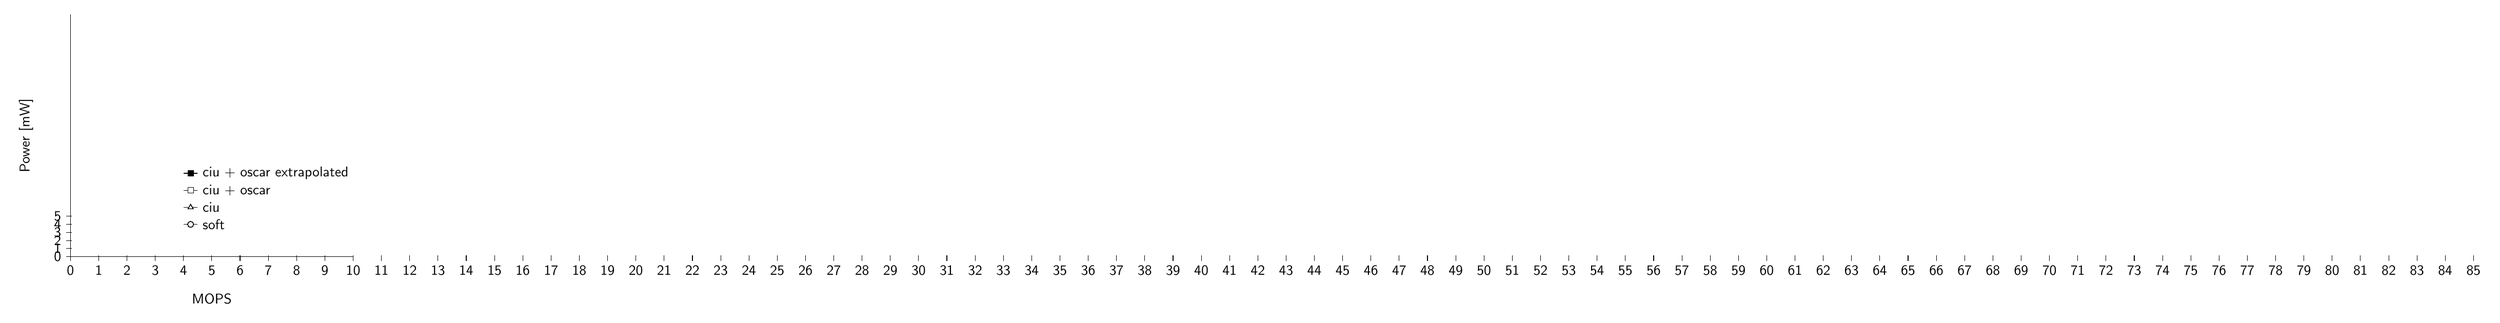
\begin{tikzpicture}[y=.2cm, x=.7cm,font=\sffamily]
 	%axis
	\draw (0,0) -- coordinate (x axis mid) (10,0);
    	\draw (0,0) -- coordinate (y axis mid) (0,30);
    	%ticks
    	\foreach \x in {0,...,85}
     		\draw (\x,1pt) -- (\x,-3pt)
			node[anchor=north] {\x};
    	\foreach \y in {0,1,...,5}
     		\draw (1pt,\y) -- (-3pt,\y) 
     			node[anchor=east] {\y}; 
	%labels      
	\node[below=0.8cm] at (x axis mid) {MOPS};
	\node[rotate=90, above=0.8cm] at (y axis mid) {Power [mW]};

	%plots
	\draw plot[mark=*, mark options={fill=white}] 
		file {plotdata/cbmc-time.dat};
	%\draw plot[mark=triangle*, mark options={fill=white} ] 
	%	file {div_ciu.dat};
	%\draw plot[mark=square*, mark options={fill=white}]
	%	file {div_ciu_oscar.dat};
	%\draw plot[mark=square*]
	%	file {div_ciu_oscar_extrapolated.dat};  
    
	%legend
	\begin{scope}[shift={(4,4)}] 
	\draw (0,0) -- 
		plot[mark=*, mark options={fill=white}] (0.25,0) -- (0.5,0) 
		node[right]{soft};
	\draw[yshift=\baselineskip] (0,0) -- 
		plot[mark=triangle*, mark options={fill=white}] (0.25,0) -- (0.5,0)
		node[right]{ciu};
	\draw[yshift=2\baselineskip] (0,0) -- 
		plot[mark=square*, mark options={fill=white}] (0.25,0) -- (0.5,0)
		node[right]{ciu + oscar};
	\draw[yshift=3\baselineskip] (0,0) -- 
		plot[mark=square*, mark options={fill=black}] (0.25,0) -- (0.5,0)
		node[right]{ciu + oscar extrapolated};
	\end{scope}
\end{tikzpicture}
\caption{\label{fig:results}
Comparison between SAT-based BMC and ACDLP: number of decisions and propagations}
\end{figure}

%
\noindent \textbf{ACDLP versus CBMC}
Fig.~\ref{fig:results} presents a comparison of the analyses using CBMC
and ACDLP.  Fig.~\ref{fig:results}(a) clearly shows that the SAT based analysis 
made significantly more decisions compared to ACDLP for all the benchmarks. 
The points on the extreme right below the diagonal in
Fig.~\ref{fig:results}(b) show that the number of propagations in the SAT based 
analysis is maximal for benchmarks that exhibit relational behaviour.  These
benchmarks are solved by octagon domain in ACDLP.  We see a reduction of at 
least two order of magnitude in the total number of decisions, propagations 
and conflicts compared to analysis using CBMC.  

Out of 85 benchmarks, SAT based analysis could prove only 26
benchmarks without any restarts.  The solver was restarted in the other 59 
cases to avoid spending too much time in ``hopeless'' branches.  By contrast, 
ACDLP solved all 85 benchmarks without restarts.  
The runtime comparison between ACDLP and CBMC are shown in 
Figure~\ref{fig:runtimes}.  ACDLP is~1.5X faster than CBMC. 
The superior performance of ACDLP is attributed to the decision heuristics, 
which exploit the high-level structure of the program, combined with the 
precise deduction by multi-way transformer and stronger learnt clause aided 
by the richer abstract domains. 
%


\noindent \textbf{ACDLP versus Astr{\'e}e}
%
To enable precise analysis using Astr{\'e}e, we manually instrument 
the benchmarks with partition directives \texttt{\_\_ASTREE\_partition\_control} 
at various control-flow joins.  These directives provides external hint to
Astr{\'e}e to guide its internal trace partition domain. 
Figure~\ref{fig:runtimes} demonstrates that Astr{\'e}e is~2X faster 
than ACDLP for {37}\% cases (32 out of 85); but the analysis using 
Astr{\'e}e shows a high degree of imprecision (marked as timeout in 
Figure~\ref{fig:runtimes}).  Astr{\'e}e reported~53 false alarms 
among~85 benchmarks.  Whereas, analysis using ACDLP produce correct 
results for all benchmarks.  Clearly, ACDLP has higher precision than 
Astr{\'e}e. Detailed analysis of the comparison between ACDLP and 
Astr{\'e}e is presented in Table~\ref{ai-result} of 
Appendix~\ref{appendix:extended_result}.  Statistics for each phase of ACDLP 
algorithm are given in Table~\ref{detailed_result} in Appendix~\ref{appendix:extended_result}.  


Our experimental evaluation suggest that ACDLP can be seen as a
technique to improve the efficiency of SAT-based BMC.  Additionally, ACDLP can
also be perceived as an automatic way to improve the precision of conventional
abstract interpretation over non-distributive lattices through automatic partition 
generation techniques such as decisions and transformer learning.
